\documentclass[10pt,a4paper]{article}
\usepackage[margin=1.0in]{geometry}

\usepackage[italian]{babel}
\usepackage{wrapfig}

\usepackage{subcaption} 

\usepackage{amsmath,amsfonts,amssymb,mathtools,gensymb}
\usepackage{enumitem}
\usepackage{graphicx}
\usepackage{booktabs,subcaption,float}
\usepackage[table]{xcolor}

% NOTE linea sottile grigia all'interno della tabella
\setlength{\lightrulewidth}{0.1pt}
\newcommand{\lightrule}{%
	\arrayrulecolor{black!30}%
	\midrule[\lightrulewidth]%
	\arrayrulecolor{black}}

\usepackage{ulem}

\graphicspath{ {./img/} }

\title{Reti: Esercizi TCP}
\author{Aymane Chabbaki}
\date{III semestre 2019/2020}

\begin{document}
	\maketitle
	\tableofcontents
	\newpage

	\section{Esame 12-6-2019}
	\begin{itemize}
		\item Un client HTTP deve trasferire da un server un file di $56200$ bytes. 
		\item Gli host (client e server) hanno i seguenti indirizzi IP 128.122.15.171/26 e 128.122.15.16/24, la tecnologia usata per la trasmissione e l'accesso alla rete è Ethernet commutata a $100$ Mbit/s dal lato client e $1$ Gbit/s dal lato server. 
		\item La rete Ethernet non è congestionata e si misura una latenza (ritardo tra l'inizio della trasmissione lato server e l'inizio della ricezione lato client) Te = $1.0$ ms. 
		\item L'overhead di Ethernet è pari a $36$ byte (includendo tutti i campi e anche l'inter-packet-gap).
	\end{itemize}
	\textbf{Domande}:
	\begin{enumerate}
		\item La consegna dei pacchetti IP avviene in modo diretto o indiretto? Perché?
		\item Che valore assume MSS (Maximum Segment Size di TCP) in assenza di opzioni per TCP e con il normale header IP (anche qui nessuna estensione o opzione viene usata)?
		\item Quanti segmenti (e quindi pacchetti IP) verranno trasmessi sulla rete?
		\item Che dimensione ha l'ultimo segmento dati della connessione?
		\item Si mostrino i segmenti scambiati per l'apertura della connessione TCP conseguente al comando di “get” da parte del client FTP, scegliendo opportunamente le porte (port number) di TCP dal lato client e dal lato server.
		\item Si mostri l'intero scambio di segmenti TCP per trasferire il file, calcolando il tempo di trasferimento e il throughput ottenuto a livello HTTP, cioè relativo ai byte utili per l'applicazione; la connessione viene chiusa dal server con un RST appena ricevuto l'ultimo ACK.
	\end{enumerate}
	La rete perde il $12 \degree$ segmento (contato ordinatamente nella segmentazione del file: i segmenti di apertura/chiusura e le ritrasmissioni non contano). Dato il basso valore di RTT, il Retransmission Timeout (RTO) di TCP è fissato al minimo ammesso dal sistema operativo: RTO $=120$ ms.
	\begin{enumerate}[resume]
		\item Si mostri nuovamente l'intero scambio di segmenti tra client e server calcolando anche il tempo di trasmissione del file e il throughput come al punto 6.
	\end{enumerate}
	\textbf{Risposte}:
	\begin{enumerate}
		\item La consegna dei pacchetti IP avviene in modo indiretto, in quanto i due indirizzi IP non appartengono alla stessa rete:
			\[
				\textnormal{IP } 128.122.15.171/26:
				\begin{cases}
					\textnormal{IP} & : 10000000.01111010.00001111.10101011 \,\,(128.122.15.171)\\
					\textnormal{SM} & : 11111111.11111111.11111111.11000000 \,\,(255.255.255.192) \\
					\textnormal{Net} & : 10000000.01111010.00001111.10000000 \,\,(128.122.15.128)
				\end{cases}
			\]
			\[
				\textnormal{IP } 128.122.15.16/24:
				\begin{cases}
					\textnormal{IP} & : 10000000.01111010.00001111.00010000 \,\,(128.122.15.16)\\
					\textnormal{SM} & : 11111111.11111111.11111111.00000000 \,\,(255.255.255.0) \\
					\textnormal{Net} & : 10000000.01111010.00001111.00000000 \,\,( 128.122.15.0)
				\end{cases}
			\]
			Visto che si hanno due indirizzi di rete diversi (128.122.15.128 e 128.122.15.0) si ha che:
			\begin{itemize}
				\item Il Client (/26) comunica indirettamente con il Server.
				\item Il Server (/24) comunica direttamente con il Client in quanto la sua rete contiene anche la sottorete del Client.
			\end{itemize}
			Questo è vero e funziona sono nel caso in cui Client e Server siano collegati ad uno Switch (se non ci fosse uno Switch, non riuscirebbero a comunicare).
		\item MSS assume il valore: $$\textrm{MSS } = 1500 - 20 - 20 = 1460 \textrm{ Byte}$$
		\item In rete vengono trasmessi (MSS = $1424$ Byte per l'overhead):
		$$ N_{s} =  \frac{56200 \textrm{ Byte}}{1424 \textrm{ Byte}} = 40 \textrm{ segmenti}$$
		\item L'ultimo segmento ha dimensione: 
		$$56200 \textrm{ Byte} - (39 \cdot 1424) \textrm{ Byte} = 56200 \textrm{ Byte} - 55536 \textrm{ Byte} = 664 \textrm{ Byte}$$
		\item TCP utilizza un meccanismo a 3 step per aprire una connessione tra sorgente e destinatario. Questa prevede che il client mandi un pacchetto speciale (con il flag SYN settato ad 1) al Server. Una volta ricevuto dal Server questo decide se accettare la domanda di connessione o rifiutarla. 
		Se la accetta, allora risponde anch'esso con un pacchetto SYN (non è un semplice SYN in quanto oltre al flag SYN ha anche il flag ACK settato così da notificare che ha ricevuto la richiesta precedentemente inviata dal Client). A questo punto il Client invia un ACK per confermare la ricezione 
		del messaggio del Server e finito questo procedimento, esiste una connessione TCP tra il Client e il Server.
		\begin{figure}[H]
			\centering
			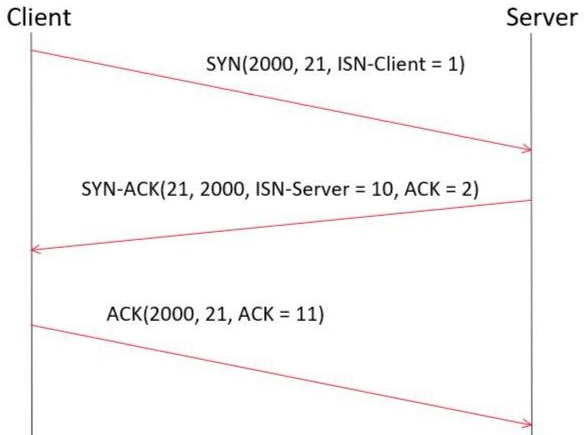
\includegraphics[width=0.5\textwidth]{ConnectionSetup_12062019}
		\end{figure}
		Il primo pacchetto SYN inviato dal Client contiene:
		\begin{itemize}
			\item Porta sorgente: 2000 (generato casualmente)
			\item Porta destinazione: 21 (porta FTP)
			\item Sequence Numerber: 1 (generato casualmente)
		\end{itemize}
		Il pacchetto SYN-ACK inviato dal Server contiene:
		\begin{itemize}
			\item Porta sorgente: 21 (porta FTP che fornisce il servizio richiesto)
			\item Porta destinazione: 2000 (porta del Client che ha richiesto il servizio)
			\item Sequence Numerber: 10 (generato casualmente)
			\item ACK: 2 (Sequence number inviato dal Client incrementato di 1 per specificare a quale pacchetto fa riferimento e ha ricevuto)
		\end{itemize}
		L'ultimo pacchetto inviato dal Client:
		\begin{itemize}
			\item Porta sorgente: 2000 
			\item Porta destinazione: 21 
			\item Sequence Numerber: 2
			\item ACK: 11 (Sequence number inviato dal Server incrementato di 1 per specificare a quale pacchetto fa riferimento e ha ricevuto)
		\end{itemize}
		\newpage
		\item Trasferimento file:
		\begin{itemize}
			\item Prima di poter disegnare il diagramma bisogna capire se si è nel caso di RTT $> T_t$ oppure $T_t > $ RTT:
			\begin{itemize}
				\item RTT $= 2 \cdot T_e = 2 \cdot 1 ms = 2ms$
				\item $T_t = \displaystyle{ \frac{1500 \textrm{ Byte}}{100 \textrm{ Mbit/s}}} =\displaystyle{ \frac{1500 \cdot 8 \textrm{ bit}}{100 \cdot 10^6 \textrm{ bit/s}}} = 120 \cdot 10^{-6} \textrm{ bit} = 0.00012 s = 0.12 ms$ 
				\item Dunque siamo nel caso in cui RTT $> T_t$
				\item In un RTT vengono trasmessi al massimo: $$\frac{\textrm{RTT}}{T_t} = \frac{2 \textrm{ ms}}{120 \mu s} = 16.67 = 16 \textrm{ segmenti} $$
				\item Questo non crea problemi (cioè i segmenti non vengono inviati back-to-back) in quanto al $6 \degree$ RTT, i segmenti che vengono trasmessi sono solo 10.
				\item Se dovessi inviare più di 10 segmenti, ad esempio 30, si ha che:
					\begin{itemize}
						\item Dal segmento 32 al 48 si è in Slow Start "normale"
						\item Dal 49 in poi, i segmenti vengono mandati back-to-back in quanto si satura completamente il numero di segmenti trasmissibili in un RTT, anche se si è ancora in Slow Start.
					\end{itemize}
			\end{itemize}
		\end{itemize}
		\begin{center}
			\centering
			 \begin{tabular}{@{} *{3}{c} @{}}
				\toprule
					\textbf{RTT} & \textbf{CWND} & \textbf{$T_w$} \\
				\midrule
					$1$ & $1$ & $[1]$ \\ 
				\lightrule
					$2$ & $2$ & $[2,3]$ \\
				\lightrule
					$3$ & $4$ & $[4,5,6,7]$ \\ 				
				\lightrule
					$4$ & $8$ & $[8,\dots,15]$ \\
				\lightrule
					$5$ & $16$ & $[16,\dots,31]$ \\
				\lightrule
					$6$ & $32$ & $[32,\dots,40]$ \\
				\bottomrule
			\end{tabular}
		\end{center}
		\begin{itemize}
			\item Il trasferimento del file: $$T_{F} = 7 \cdot RTT = 7 \cdot (2 \cdot T_e) = 14 \cdot 1 \,ms = 14 \,ms$$
			\item Throughput: $$T_h = \displaystyle{\frac{56200 \textrm{ Byte}}{T_F} = \frac{449600 \textrm{ bit}}{14 ms} = \frac{449600 \textrm{ bit}}{0.014 s} = 32114285.7 \textrm{ bit/s} = 30.6 \textrm{ Mbit/s}}$$
		\end{itemize}
	\newpage
	\item Trasmissione con il $12 \degree$ pacchetto perso:
	\begin{itemize}
		\item RTO = $120 ms$, SSTHR = $64$ Kbyte $= 45$ segmenti.
		\item Il trasferimento parte con Slow Start con CWND = 1. Dopo un RTT, la finestra di trasmissione raddoppia e possono partire i pacchetti S2 e S3. Dopo un altro RTT, la finestra di trasmissione raddoppia nuovamente e vengono inviati i pacchetti S3,S4,S5,S6,S7.
		\item Al terzo RTT, la finestra di trasmissione è di 8 segmenti, i segmenti S8-S11 vengono trasmessi correttamente; il segmento S12 viene perso.
		\item Vengono trasmessi successivamente i segmenti S13-S15, ma visto che il Client è fermo ancora al segmento S11 e si aspetta S12, manda 3 ACK duplicati.
		\item Questo fa si che si passi in Fast Recovery (SSTHR = CWND/2 = 12/2 = 6, CWND = SSTHR + 3 = 9, Tw = [12,13,14,15,16,17], recovery = 23). Viene ritrasmesso il segmento S12 (non vengono trasmessi altri segmenti in quanto la finestra di trasmissione non contiene segmenti nuovi da trasmettere).
		\item I segmenti S16-S23 vengono ricevuti dal Client, ma ritorna per ognuno di questi segmenti un ACK duplicato notificando al Server che è in attesa di S12. Questi 8 ACK duplicati fanno si che la dimensione della finestra di trasmissione aumenti di 8 (Tw = [12,...,28]). La finestra di trasmissione mi permette di trasmettere i segmenti S24-S28.
		\item Il Client riceve il segmento S12 e trasmette un ACK cumulativo (A23) al Server, notificando che ha ricevuto correttamente fino al segmento S23.
		\item Ricevuto questo ACK, il Server esce da Fast Recovery e passa a Congestion Avoidance (CWND = SSTHR = 6, Tw = [24,...,29]) e posso trasmettere il segmento S29.
		\item La trasmissione continua con Congestion Avoidance fino alla trasmissione e recezione dell'ACK del segmento S40 (da notare che quando il Server riceve l'ACK A29, la dimensione finestra di trasmissione aumenta da 5 a 6).
		\item Il Server una volta ricevuto l'ACK A40 relativo al segmento S40, trasmette un ultimo segmento (con il flag RST settato) così da terminare la connessione con il Client.
	\end{itemize}
	\newpage
	\begin{figure}[H]
		\begin{subfigure}[b]{9cm}
		  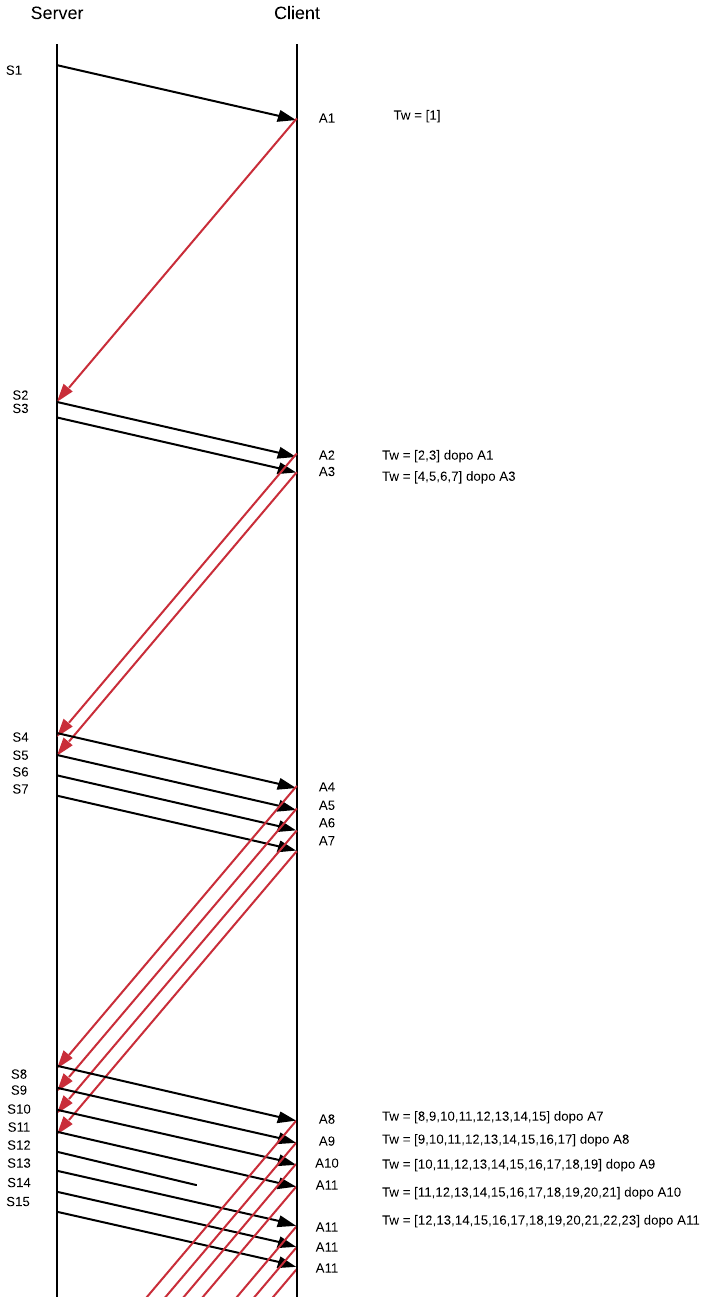
\includegraphics[width=\textwidth]{Esame1262019_Conperdite1}
		\end{subfigure}
		\begin{subfigure}[b]{9cm}
		  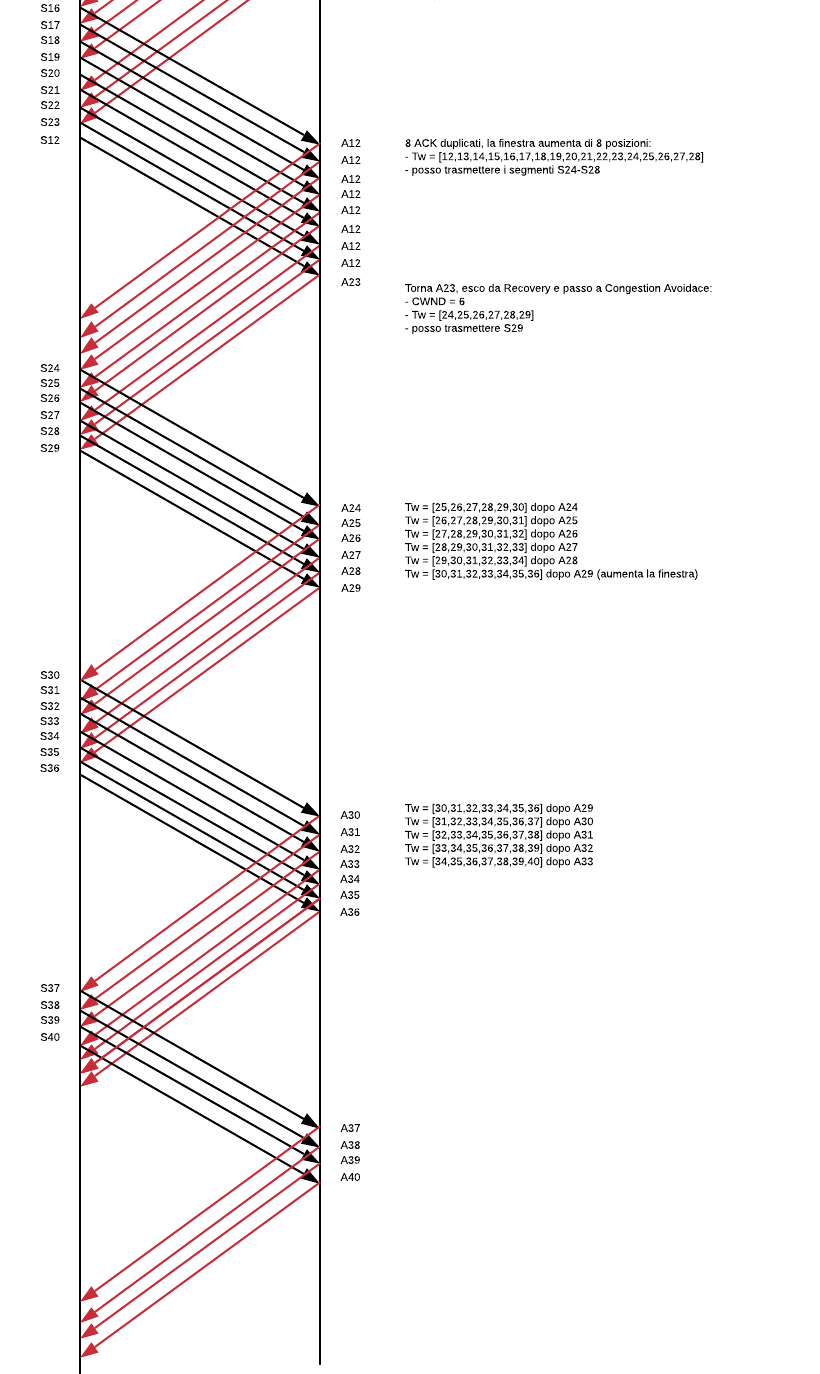
\includegraphics[width=\textwidth]{Esame1262019_Conperdite2}
		\end{subfigure}
	  \end{figure}
	\end{enumerate}

	\newpage

	\section{Esame 11-01-2019}
	\begin{itemize}
		\item Consideriamo una applicazione web basata su http $1.1.$ Il browser del Client consente l'apertura di 2 connessioni TCP persistenti in parallelo. 
		\item Client e Server sono connessi a una stessa subnet IP, realizzata su una LAN Ethernet a $100$ Mbit/s. 
		\item Il tempo di propagazione tra Client e Server, inclusi gli switch Ethernet, è approssimativamente costante e pari a $200 \mu s$. 
		\item Entrambe le Receiver Windows (RCWND) sono pari a $64$ KByte.
		\item Durante una sessione, il Client richiede il trasferimento di $5$ piccoli oggetti (file) di dimensioni rispettivamente:
			\begin{itemize}
				\item O1 = $4500$ Byte
				\item O2 = $11400$ Byte
				\item O3 = $7800$ Byte
				\item O4 = $9400$ Byte
				\item O5 = $13200$ Byte
			\end{itemize}
		\item Si assuma che le connessioni TCP si comportino come se fossero appena state aperte.
	\end{itemize}
	\textbf{Domande:}
	\begin{enumerate}
		\item Come viene suddiviso il trasferimento dei 5 oggetti sulle 2 connessioni? Esiste una soluzione unica oppure sceglie il browser?
		\item Mostrare in un diagramma lo scambio dei segmenti su una delle due connessioni a scelta, chiamiamola C.
		\item La perdita di pacchetti su una connessione influenza il comportamento dell'altra?
		\item Mostrare in un diagramma lo scambio dei segmenti sulla connessione C nel caso in cui la LAN scarti il $7 \degree$ pacchetto trasmesso.
		\item Calcolare il tempo di trasferimento totale dei cinque oggetti in assenza di perdite (bisogna tenere in conto entrambe le connessioni, ovviamente). Si trascurino gli header di http e altre informazioni che il server potrebbe aggiungere ai 5 file; si deve invece considerare l'overhead introdotto da TCP/IP e da Ethernet. Si consideri per quest'ultimo un header 
		equivalente (incluso l'Inter Packet Gap) di $38$ Byte.
		\item Supponiamo ora che il sistema operativo consenta l'apertura di 1 sola connessione e non di 2; ricalcolare il tempo di trasmissione totale dei 5 oggetti.
		\item Commentare alla luce dello scenario dato i risultati ottenuti ai punti 5 e 6.
	\end{enumerate}
	\textbf{Risposte:}
	\begin{enumerate}
		\item Il trasferimento è gestito dal Browser, che decide autonomamente come trasferire i pacchetti usando le due connessioni a disposizione.
		\item Dati utili per la risoluzione dell'esercizio:
		\begin{itemize}
			\item I 5 file da trasferire hanno dimensione totale: $$D = (4500 + 11400 + 7800 + 9400 + 13200) \textrm{ Byte} = 46300 \textrm { Byte}$$
			\item MSS = $1500 - 20 - 20 = 1460$ Byte
			\item Il numero di segmenti da trasferire: $$S_t = \frac{46300 \textrm{ Byte}}{1460 \textrm{ Byte}} = 31.7 = 32\textrm{ segmenti}$$
			\item L'ultimo segmento ha dimensione: $$46300 - (31 \cdot 1460) = 46300 - 45260 = 1040 \textrm{ Byte}$$
			\item Calcolo il tempo di trasmissione: $$T_t = \frac{8 \cdot 1500 \textrm{ bit}}{100  \cdot 10^6 \textrm{ bit/s}} = 0.00012 s = 120 \mu s$$
			\item Sapendo che il tempo di propagazione tra Client e Server è pari a $200 \mu s$ e che: $$\textrm{RTT} = 2 \cdot 200 \mu s = 400 \mu s$$
			\item Siamo nel caso in cui $\textrm{RTT} > T_t$:
			\begin{itemize}
				\item In un RTT vengono trasmessi al massimo: $$\frac{\textrm{RTT}}{T_t} = \frac{400 \mu s}{120 \mu s} = 3.33 = 3 \textrm{ segmenti}$$
				\item $\textrm{RCWND} = \displaystyle{\frac{64 \text{ KByte}}{1460 \textrm{ Byte}} = \frac{65536 \text{ Byte}}{1460 \textrm{ Byte}} = 45 \textrm{ segmenti}}$
				\item $\textrm{SSTHR} = \textrm{RCWND} = 45 \textrm{ segmenti}$
				\item $\textrm{RTO} = 1s$
				\item $\textrm{CWND} = 1$
				\item Scambio dei pacchetti:
				\begin{figure}[H]
					\centering
					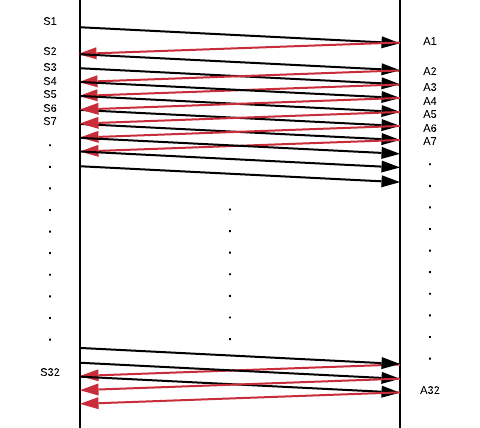
\includegraphics[width=10cm]{Esame1112019_Senzaperdite}
				\end{figure}
				\item Tempo di trasmissione:
				$$T = \frac{8 \cdot (24 \cdot 1500 + 1080) \textrm{ bit}}{ 100 \cdot 10^6 \textrm{ bit/s}} + 3 \textrm{ RTT} = 2966.4 \mu s + 1200 \mu s = 4166.4 \mu s = 4.2 ms$$
			\end{itemize}
		\end{itemize}
		\item Non influenza direttamente, quello che succede se una connessione perde pacchetti è che causa un ritardo all'altra connessione, in quanto il traffico non può transitare contemporaneamente nelle due connessioni, sennò si rischiano delle collisioni.
		\item Nel caso venga perso il $7 \degree$ pacchetto:
			\begin{figure}[H]
				\centering
				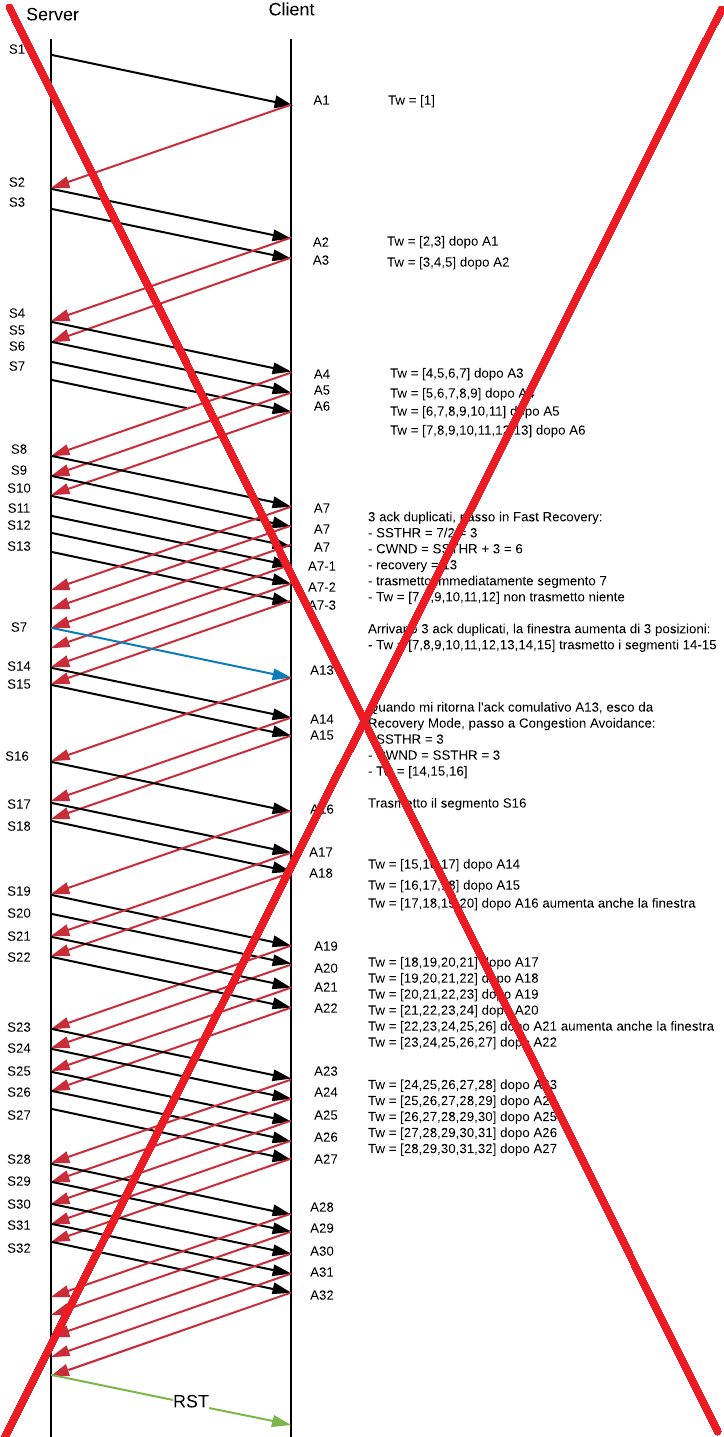
\includegraphics[width=9.5cm]{Esame1112019_Conperdite}
			\end{figure}
		\item Complicato e non visto a lezione.
		\item Il tempo è uguale a quello calcolato nell'esercizio 2.
	\end{enumerate}

	\newpage

	\section{Esame 08-01-2018}
	\begin{itemize}
		\item Un client HTTP deve trasferire da un server un file di $42800$ Bytes. 
		\item Gli host (client e server) hanno i seguenti indirizzi IP 130.122.15.171/24 e 130.122.1.4/24, la tecnologia usata per la trasmissione e l'accesso alla rete è Ethernet commutata a $100$ Mbit/s dal lato client e $1$ Gbit/s dal lato server. 
		\item La rete Ethernet non è congestionata e si misura una latenza (ritardo tra l'inizio della trasmissione lato server e l'inizio della ricezione lato client) Te $= 1.2 ms$. 
		\item L'overhead di Ethernet è pari a $36$ Byte (includendo tutti i campi e anche l'inter-packet-gap).
	\end{itemize}
	\textbf{Domande}:
	\begin{enumerate}
		\item La consegna dei pacchetti IP avviene in modo diretto o indiretto? Perché?
		\item Che valore assume MSS (Maximum Segment Size di TCP) in assenza di opzioni per TCP e con il normale header IP (anche qui nessuna estensione o opzione viene usata)?
		\item Quanti segmenti (e quindi pacchetti IP) verranno trasmessi sulla rete?
		\item Che dimensione ha l'ultimo segmento dati della connessione?
		\item Si mostrino i segmenti scambiati per l'apertura della connessione TCP conseguente al comando di “get” da parte del client FTP, scegliendo opportunamente le porte (port number) di TCP dal lato client e dal lato server.
		\item Si mostri l'intero scambio di segmenti TCP per trasferire il file, calcolando il tempo di trasferimento e il throughput ottenuto a livello HTTP; la connessione viene chiusa dal server con un RST appena ricevuto l'ultimo ACK.
	\end{enumerate}
	La rete perde il $15 \degree$ segmento (contato ordinatamente nella segmentazione del file: i segmenti di apertura/chiusura e le ritrasmissioni non contano). Dato il basso valore di RTT, il Retransmission Timeout (RTO) di TCP è fissato al minimo ammesso dal sistema operativo: RTO $=180ms$.
	\begin{enumerate}[resume]
		\item Si mostri nuovamente l'intero scambio di segmenti tra client e server calcolando anche il tempo di trasmissione del file e il throughput come al punto 6.
	\end{enumerate}
	\textbf{Risposte}:
	\begin{enumerate}
		\item La consegna dei pacchetti IP avviene in modo indiretto, in quanto i due indirizzi IP non appartengono alla stessa rete:
			\[
				\textnormal{IP } 130.122.15.171/24:
				\begin{cases}
					\textnormal{IP} & : 10000010.01111010.00001111.10101011 \,\,(130.122.15.171)\\
					\textnormal{SM} & : 11111111.11111111.11111111.00000000 \,\,(255.255.255.0) \\
					\textnormal{Net} & : 10000010.01111010.00001111.00000000 \,\,(130.122.15.0)
				\end{cases}
			\]
			\[
				\textnormal{IP } 130.122.1.4/24:
				\begin{cases}
					\textnormal{IP} & : 10000010.01111010.00000001.00000100 \,\,(130.122.1.4)\\
					\textnormal{SM} & : 11111111.11111111.11111111.00000000 \,\,(255.255.255.0) \\
					\textnormal{Net} & : 10000010.01111010.00000001.00000000 \,\,(130.122.1.0)
				\end{cases}
			\]
			Visto che si hanno due indirizzi di rete diversi (130.122.1.0 e 130.122.15.0) allora Client e Server non comunicano direttamente, ma dovranno comunicare tramite un router.
		\item In assenza di opzioni per TCP e con il normale header IP, MSS assume valore: $$\textrm{MSS} = \textrm{MTU} - 20 \textrm{ Byte} - 20 \textrm{ Byte} = 1500 \textrm{ Byte} - 40 \textrm{ Byte} = 1460 \textrm{ Byte}$$
		\item Visto che abbiamo un overhead di $36$ Byte, si ha che MSS = $1424$ Byte; dunque il numero di segmenti che verranno trasmessi è:
		$$S_F = \frac{42800 \textrm{ Byte}}{1424 \textrm{ Byte}} = 30.05 = 31 \textrm{ segmenti}$$
		\item L'ultimo pacchetto ha dimensione: $42800 - (30 \cdot 1424) = (42800 - 42720) = 80 \textrm{ Byte}$
		\item TCP utilizza un meccanismo a 3 step per aprire una connessione tra sorgente e destinatario. Questa prevede che il client mandi un pacchetto speciale (con il flag SYN settato ad 1) al Server. Una volta ricevuto dal Server questo decide se accettare la domanda di connessione o rifiutarla. 
		Se la accetta, allora risponde anch'esso con un pacchetto SYN (non è un semplice SYN in quanto oltre al flag SYN ha anche il flag ACK settato così da notificare che ha ricevuto la richiesta precedentemente inviata dal Client). A questo punto il Client invia un ACK per confermare la ricezione 
		del messaggio del Server e finito questo procedimento, esiste una connessione TCP tra il Client e il Server.
			\begin{figure}[H]
				\centering
				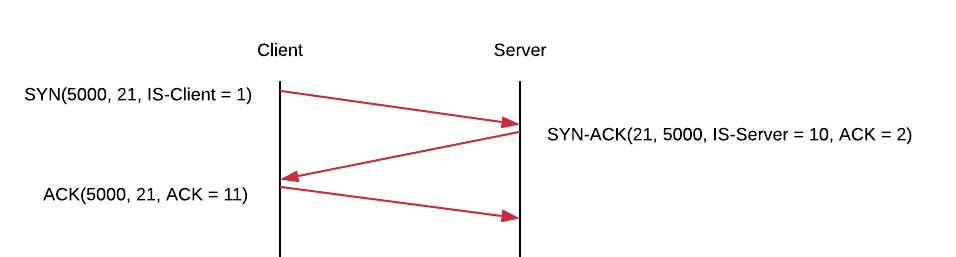
\includegraphics[width=15cm]{Esame812019_FTPHandshake}
			\end{figure}
			Il primo pacchetto SYN inviato dal Client contiene:
			\begin{itemize}
				\item Porta sorgente: 5000 (generato casualmente)
				\item Porta destinazione: $21$ (porta FTP)
				\item Sequence Numerber: $1$ (generato casualmente)
			\end{itemize}
			Il pacchetto SYN-ACK inviato dal Server contiene:
			\begin{itemize}
				\item Porta sorgente: $21$ (porta FTP che fornisce il servizio richiesto)
				\item Porta destinazione: $5000$ (porta del Client che ha richiesto il servizio)
				\item Sequence Numerber: $10$ (generato casualmente)
				\item ACK: $2$ (Sequence number inviato dal Client incrementato di $1$ per specificare a quale pacchetto fa riferimento e ha ricevuto)
			\end{itemize}
			L'ultimo pacchetto inviato dal Client:
			\begin{itemize}
				\item Porta sorgente: $5000$ 
				\item Porta destinazione: $21$ 
				\item Sequence Numerber: $2$
				\item ACK: 11 (Sequence number inviato dal Server incrementato di $1$ per specificare a quale pacchetto fa riferimento e ha ricevuto)
			\end{itemize}
		\item Trasferimento file:
			\begin{itemize}
				\item Prima di poter disegnare il diagramma bisogna capire se si è nel caso di RTT $> T_t$ oppure $T_t > $ RTT:
				\begin{itemize}
					\item RTT $= 2 \cdot T_e = 2 \cdot 1.2 ms = 2.4ms$
					\item $T_t = \displaystyle{ \frac{1500 \textrm{ Byte}}{100 \textrm{ Mbit/s}}} =\displaystyle{ \frac{1500 \cdot 8 \textrm{ bit}}{100 \cdot 10^6 \textrm{ bit/s}}} = 120 \cdot 10^{-6} \textrm{ bit} = 0.00012 s = 0.12 ms$ 
					\item Dunque siamo nel caso in cui RTT $> T_p$
						\begin{itemize}
							\item In un RTT vengono trasmessi al massimo: $$\frac{\textrm{RTT}}{T_t} = \frac{2.4 ms}{0.12 ms} = 20 \textrm{ segmenti}$$
						\end{itemize}
				\end{itemize}
			\end{itemize}
			\begin{center}
				\centering
 				\begin{tabular}{@{} *{3}{c} @{}}
					\toprule
						\textbf{RTT} & \textbf{CWND} & \textbf{$T_w$} \\
					\midrule
						$1$ & $1$ & $[1]$ \\ 
					\lightrule
						$2$ & $2$ & $[2,3]$ \\
					\lightrule
						$3$ & $4$ & $[4,5,6,7]$ \\ 				
					\lightrule
						$4$ & $8$ & $[8,\dots,15]$ \\
					\lightrule
						$5$ & $16$ & $[16,\dots,31]$ \\
					\bottomrule
				\end{tabular}
			\end{center}
			\begin{itemize}
				\item Il trasferimento del file: $$T_{F} = 6 \cdot RTT = 6 \cdot (2 \cdot T_e) = 12 \cdot 1.2 \,ms = 14.4 \,ms$$
				\item Throughput: $$T_h = \displaystyle{\frac{42800 \textrm{ Byte}}{T_F} = \frac{342400 \textrm{ bit}}{14.4 ms} = \frac{342400 \textrm{ bit}}{0.0144 s} = 23777777.7 \textrm{ bit/s} = 22.7 \textrm{ Mbit/s}}$$
			\end{itemize}
		\item Trasmissione con il $15 \degree$ pacchetto perso:
			\begin{itemize}
				\item RTO = $180 ms$
				\item SSTHR = $64$ Kbyte $= 44$ segmenti.
				\item Il trasferimento parte con Slow Start con CWND = 1.
				\item Dopo un RTT, la finestra di trasmissione raddoppia e vengono trasmessi i segmenti S2 e S3.
				\item Dopo un altro RTT, la finestra raddoppia nuovamente e vengono inviati i pacchetti S3,S4,S5,S6,S7.
				\item Al terzo RTT, la finestra è di 8 segmenti e l'ultimo pacchetto che viene trasmesso è il $15 \degree$, che viene perso.
				\item Gli ACK dei segmenti trasmessi prima del pacchetto S15 vengono ricevuti dal Client, che aumenta la finestra di trasmissione (CWND = [15-29]) ma il Server non riceve l'ACK del segmento A15.
				\item Il Server trasmette i segmenti non inviati della finestra di trasmissione e dopo un RTT inizia a ricevere gli ACK dal Client.
				\item Visto che il segmento S15 non è stato ricevuto dal Client, il Server riceve 3 ACK duplicati dei segmenti S16-S18 (viene notificato del fatto che il Client ha ricevuto fino al S14 pacchetto).
				\item TCP entra in fase Fast recovery (dimezza SSTHR, inizializza CWND a SSTHR e la incrementa di 3, salva nella variabile recovery A29 che è l'ultimo pacchetto che il Server ha inviato).
				\item Viene trasmesso il pacchetto perso (S15); la nuova finestra non permette la trasmissione di nuovi segmenti (sono già stati trasmessi tutti).
				\item Vengono ricevuti dal Server 11 ACK duplicati (A20-A29), seguendo l'algoritmo di Fast Retransmit, la finestra del Server viene incrementa di 11 posizioni (Tw = [15,...,31]).
				\item Visto che la finestra lo permette, il Server è abilitato a trasmettere i segmenti S30 e S31.
				\item Quando il Client riceve S15, manda un ACK cumulativo notificando al Server che ha ricevuto tutto fino al segmento S29.
				\item Una volta ricevuto questo ACK, il Server esce dalla modalità Fast Recovery e passa a Congestion Avoidance (setta CWND = SSTHR = 7).
				\item La nuova finestra non permette al Server di inviare nessun nuovo segmento, in quanto sono già stati tutti trasmessi; dunque aspetta gli ACK dei segmenti che ha trasmesso, così per poter chiudere la connessione.
				\item Ricevuti gli ultimi ACK, il Server manda un ultimo segmento, con il flag RST settato, così chiude la connessione con il Client.
			\end{itemize}
			\newpage
			\begin{figure}[H]
				\begin{subfigure}[b]{9cm}
				  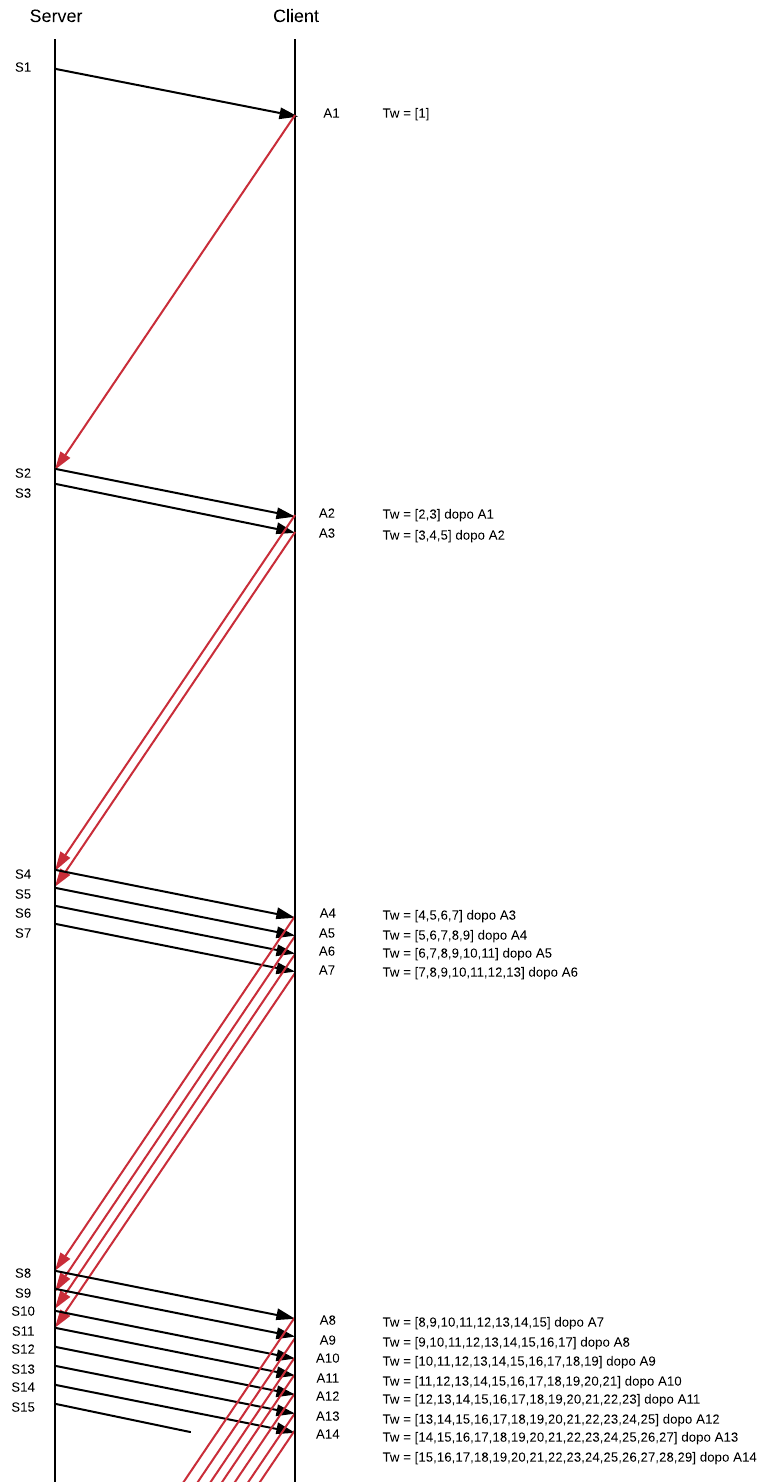
\includegraphics[width=\textwidth]{Esame812019_Conperdite1}
				\end{subfigure}
				\begin{subfigure}[b]{9cm}
				  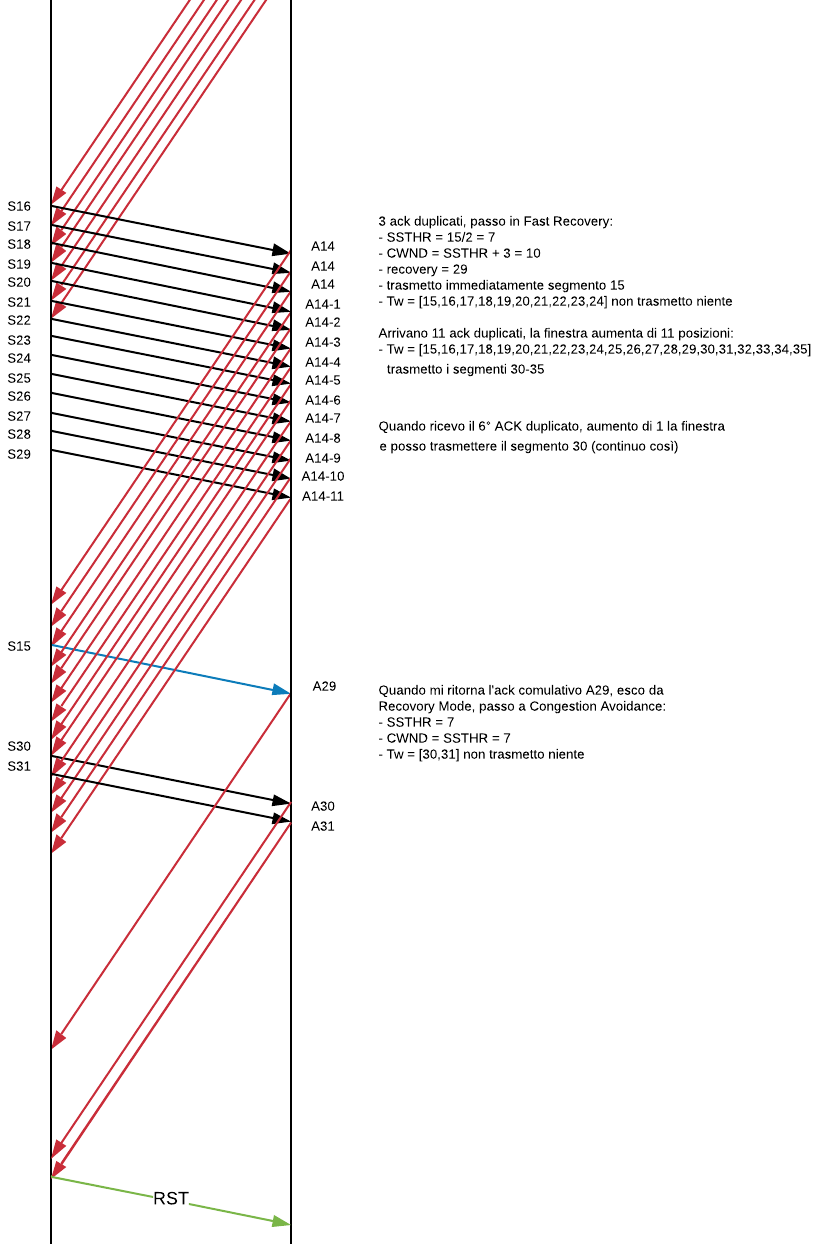
\includegraphics[width=\textwidth]{Esame812019_Conperdite2}
				\end{subfigure}
			  \end{figure}
	\end{enumerate}
\end{document} 